\section{Data Model}%
\label{data-model}

While datatypes introduced by computer architectures and software
libraries are important for the data model, they are discussed
separately in .

The data model of a system organizes elements of data, standardizes how
they represent data entities and how users can interact with the data.
The \textbf{model} can be split into three layers:

\begin{itemize}
  \item The \textbf{conceptual data} model describes the entities and the
    semantics of the domain that are represented by the data model and the
    typical operations to manipulate the data. In our case, the scientific
    domain is NWP/climate.
  \item The \textbf{logical data model} describes the abstraction level
    provided by the system, how domain entities are mapped to objects
    provided by the system\footnote{A entity of the domain model such as a
    car could be mapped to one or several objects.}, and the supported
    operations to access and manipulate these objects are defined.
    Importantly, the \textbf{logical data model} defines the semantics
    when using the operations to access and manipulate the system objects.
    For example, a system object of a relational model is a table --
    representing attributes of a set of objects -- and a row of a table
    representing attributes of a single object.
  \item The physical data model describes how the logical entities are finally
    mapped to objects/files/regions on available hardware. The physical
    data model is partly covered by the backends of ESDM, therefore, the
    descriptions will stop at that abstraction level.
\end{itemize}

\subsection{Conceptual Data Model}

Our conceptual data model is aligned with the needs of domain scientists
from climate and weather. It reuses and extends from concepts introduced
in a data model proposed for the Climate and Forecasting conventions for
NetCDF data.
%\footnote{\href{\%22A\%20CF\%20Data\%20Model\%20and\%20Implementation\%22,\%20Hassel\%20et\%20al,\%202017,\%20GMD\%20submitted}{"A CF Data Model and Implementation", Hassel et al, 2017, GMD submitted}}.

\paragraph{Variable:}%
\label{variable}

A variable, \(V\), defines a set of data representing a discrete
(generally scalar) quantity discretised within a ``sampling'' domain,
\(d\). It is accompanied by

\paragraph{Metadata:}%
\label{metadata}

Which will include at the minimum, a name, but may also include units,
and information about additional dimensionality, directly (e.g.~via a
key, value pair such as that necessary to expose \(z=1.5m\) for air
temperature at 1.5m) or indirectly (e.g.~via pointers to other generic
coordinate variables which describe the sampled domain). There may also
be a dictionary of additional metadata which may or may not conform to
an external semantic convention or standard. Such metadata could include
information about the tool used to observe or simulate the specific
variable. Additional metadata is also required for all the other
entities described below.

\paragraph{Dimension:}%
\label{dimension}

The sampling domain \(d\) is defined by Dimensions which define an a
coordinate axis. Dimensions will also include metadata, which must
again, include at a minimum a name (e.g.~height, time), but may also
include information about directionality, units (e.g.~degrees, months,
days-since-a-particular-time-using-a-particular-calendar), or details of
how to construct an algorithm to find the actual sampling coordinates,
perhaps using a well known algorithm such as an ISO 8601 time.

\paragraph{Coordinate:}%
\label{coordinate}

Coordinates are the set of values at which data is sampled along any
given dimension. They may be explicitly defined by indexing into a
coordinate variable, or implicitly defined by an algorithm. When we talk
about the coordinates, it is usually clear if we mean the N-dimensional
coordinate to address data in a given variable or if we just mean the
(1D) coordinate along one dimension.

\paragraph{Cell:}%
\label{cell}

The data values are known at points, which may or may not represent a
cell. Such cells are n-dimensional shapes where the dimensionality may
or may not fully encompass the dimensionality of the domain.
n-dimensional shapes can be implicitly defined in which case the
Cartesian product of all dimensional coordinates forms the data "cube"
of the cell, but they can also be explicitly defined, either by
providing bounds on the coordinate variables (via metadata) or by
introducing a new variable which explicitly defines the functional
boundaries of the cell (as might happen in a finite element unstructured
grid).

\paragraph{Dataset:}%
\label{dataset}

Variables can be aggregated into datasets. A dataset contains multiple
variables that logically belong together, and should be associated with
metadata describing the reason for the aggregation. Variables must have
unique names within a dataset.

Our conceptual model assumes that all variables are scalars, but clearly
to make use of these scalars requires more complex interpretation. In
particular, we need to know the

\paragraph{Datatype:}%
\label{datatype}

which defines the types of values that are valid and the operations that
can be conducted. While we are mostly dealing with scalars, they may not
be amenable to interpretation as simple numbers. For example, a variable
may be storing an integer which points into a taxonomy of categories of
land-surface-types. More complex structures could include complex data
types such as vectors, compressed ensemble values, or structures within
this system, provided such interpretation is handled outside of the
ESDM, and documented in metadata. This allows us to limit ourselves to
simple data types plus arbitrary length blocks of bits.

\paragraph{Operators:}%
\label{operators}

Define the manipulations possible on the conceptual entities. The
simplest operators will include creation, read, update and delete
applied to an entity as a whole, or to a subset, however even these
simple operators will come with constraints, for example, it should not
be possible to delete a coordinate variable without deleting the parent
variable as well. There will need to be a separation of concerns between
operators which can be handled \emph{within} the ESDM subsystem, and
those which require external logic. Operators which might require
external logic could include subsetting --- it will be seen that the
ESDM will support simple subsetting using simple coordinates --- but
complex subsets such as finding a region in real space from dimensions
spanned using an algorithm or coordinate variable, may require knowledge
of how such algorithms or variables are specified. Such knowledge is
embedded in conventions such as the CF NetCDF conventions, and this
knowledge could only be provided to the ESDM via appropriate operator
plugins.

\subsection{Logical Data Model}

The logical data model describes how data is represented inside ESDM,
the operations to interact with the data and their semantics. There are
four first class entities in the ESDM logical data model:
\textbf{variable}s, \textbf{fragment}s, \textbf{container}s, and
\textbf{metadata}. ESDM entities may be linked by ESDM
\textbf{reference}s, and a key property which emerges from the use of
references is that no ESDM entity instance may be deleted while
references to it still exist. The use of reference counting will ensure
this property as well as avoid dangling pointers.

gives an overview of the logical data model.

Each of these entities is now described, along with a list of supported
operations:

\paragraph{Variable:}%
\label{variable-1}

In the logical data model, the variable corresponds directly to a
variable in the conceptual data model. Each element of the variable
sampled across the dimensions contains data with a prescribed
\textbf{DataType}. Variables are associated with both \textbf{Scientific
Metadata} and \textbf{Technical Metadata}. Variables are partitioned
into \textbf{fragments} each of which can be stored on one or more
``storage backend.'' A variable definition includes internal information
about the domain (bounding box in some coordinate system) and
dimensionality (size and shape), while the detailed information about
which coordinate variables are needed to span the dimensions and how
they are defined is held in the technical metadata. Similarly, where a
variable is itself a coordinate variable, a link to the parent variable
for which it is used is held in the technical metadata. The ESDM will
not allow an attempt to delete a variable to succeed while any such
references exist (see references). A key part of the variable definition
is the list of fragments associated with it, and if possible, how they
are organised to span the domain. Users may choose to submit code pieces
that are then run within the I/O-path (not part within ESiWACE
implementation), such an operation covers the typical filter, map and
reduce operations of the data flow programming paradigm.

Fragments are created by the backend while appending/modifying data to a
variable.

Operations:

\begin{itemize}
  \item Variables can be created and deleted.
  \item Fragments of data can be attached and deleted.
  \item Fragments can be repartitioned and reshuffled.
  \item Integrity can be checked.
  \item Data can be read, appended or modified those operations will be translated to the responsible fragments.
  \item Metadata can be atomically attached to a variable or modified.
  \item A variable can be sealed to make it immutable for all subsequent modifications.
  \item Process data of the variable somewhere in the I/O-path.
\end{itemize}

\paragraph{Fragment:}%
\label{fragment}

A fragment is a piece (subdomain) of a variable. The ESDM expects to
handle fragments as atomic entities, that is, only one process can write
a fragment through the ESDM, and the ESDM will write fragments as atomic
entities to storage backends. The backends are free to further partition
these fragments in an appropriate way, for example, by sharding using
chunks as described in the mapping section. However, the ESDM is free to
replicate fragments or subsets of fragments and to choose which backend
is appropriate for any given fragment. This allows, for example, the
ESDM to split a variable into fragments some of which are on stored on a
parallel file system, while others are placed in object storage.

Operations:

\begin{itemize}
  \item Data of fragments can be read, appended or modified.
  \item Integrity of the fragment can be checked.
  \item Process data of the variable somewhere in the I/O-path.
\end{itemize}

\paragraph{Container:}%
\label{container}

A container is a virtual entity providing views on collections of
variables, allowing multiple different datasets (as defined in the
conceptual model) to be realised over the variables visible to the ESDM.
Each container provides a hierarchical namespace holding references to
one or multiple variables together with metadata. Variables cannot be
deleted while they are referenced by a container. The use of these
dynamic containers provides support for much more flexible organisation
of data than provided by a regular file system semantics --- and
efficiently support high level applications such as the Data Reference
Syntax\footnote{Taylor et al (2012): CMIP5 Data Reference Syntax (DRS) and Controlled Vocabularies.}.

A container provides the ESDM storage abstraction which is analogous to
an external file. Because many scientific metadata conventions are based
on semantic structures which span variables within a file in ways that
may be opaque to the ESDM without the use of a plugin, the use of a
container can indicate to the ESDM that these variables are linked even
though the ESDM does not understand why, and so they cannot be
independently deleted. When entire files in NetCDF format are ingested
into the ESDM, the respective importing tool must create a container to
ensure such linking properties are not lost.

Operations:

\begin{itemize}
  \item Creation and deletion of containers.
  \item Creation and deletion of names in the hierarchical name space; the creation of links to an existing variable.
  \item Attaching and modification of metadata.
  \item Integrity can be checked.
\end{itemize}

\paragraph{Metadata:}%
\label{metadata-1}

Can be associated with all the other first class entities (variables,
fragments, and containers). Such metadata is split into internal ESDM
technical metadata, and external user-supplied semantic metadata.

Technical metadata covers, e.g., permissions, information about data
location and timestamps. A backend will be able to add its own metadata
to provide the information to lookup the data for the fragment from the
storage backend managed by it. Metadata by itself is treaded like a
normal ESDM variable but linked to the variable of choice. The
implementation may embed (simple) metadata into fragments of original
data (see Reference).

Operations:

\begin{itemize}
  \item Uses can create, read, or delete arbitrary scientific metadata onto
    variables and containers. A future version of the ESDM may support
    user scientific metadata for fragments.
  \item Container level metadata is generally not directly associated with
    variables, but may be retrieved via following references from
    variables to containers.
  \item Queries allow to search for arbitrary metadata, e.g., for objects that
    have (\texttt{experiment=X,\ model=Y,\ time=yesterday}) returning the
    variables and containers in a list that match. This enables to locate
    scientific data in an arbitrary namespace.
\end{itemize}

\paragraph{Reference:}%
\label{reference}

A reference is a link between entities and can be used in many places,
references can be embedded instead of real data of these logical
objects. For example, dimensions inside a variable can be references,
also a container typically uses references to variables.

Operations:

\begin{itemize}
  \item A reference can be created from existing logical entities or removed.
\end{itemize}

%\begin{figure}
%  \centering
%  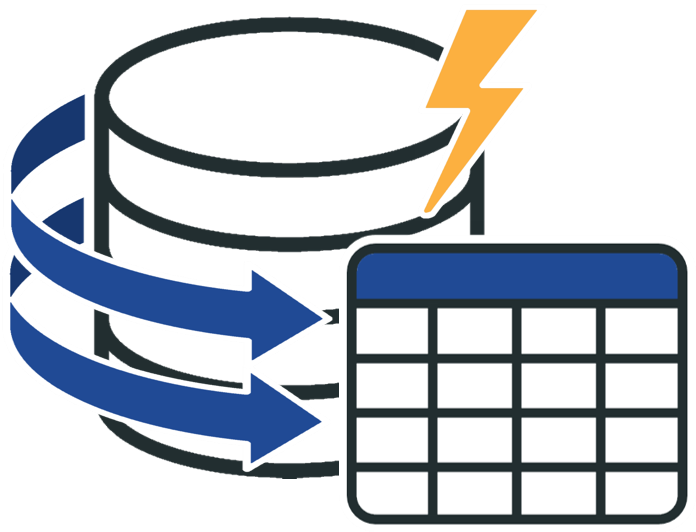
\includegraphics[width=0.5\textwidth]{../figures/data-model.png}
%  \caption{Logical Data Model (TODO)}%
%  \label{fig:data-model}
%\end{figure}

\paragraph{Namespace:}%
\label{namespace}

ESDM does not offer a simple hierarchical namespace for the files. It
provides the elementary functions to navigate data: teleportation and
orientation in the following fashion: Queries about semantical data
properties (e.g.,
\texttt{experiment=myExperiment,\ model=myModel,\ date=yesterday}) can
be performed returning a list of matching files with their respective
metadata. Iterating the list (orientation) is similar to listing a
directory in a file system.

Note that this reduces the burden to define a hierarchical namespace and
for data sharing services based on scientific metadata. An input/output
container for an application can be assembled on the fly by using
queries and name the resulting entities. As a container provides a
hierachical namespace, by harnessing this capability one can search for
relevant variables and map them into the local file system tree,
accessing these variables as if they would be, e.g., NetCDF files. By
offering a FUSE client, this feature also enables backwards
compatibility for legacy POSIX applications.
